\section{Autenticazione e gestione profilo}

	\subsection{Registrazione}
	\label{registrazione}

	Il primo passo per poter utilizzare l'applicazione MaaP è la registrazione. \`E possibile registrasi cliccando sul link \texttt{Sign up} presente nella homepage. Verrà proposto un \glossario{form} da compilare con \texttt{email} e \texttt{password}, dopodiché bisognerà proseguire cliccando il pulsante \texttt{Sign up}.

	\subsection{Autenticazione}
	\label{autenticazione}
	Per poter effettuare il login è necessario essere registrati (vedi \ref{registrazione}). Il login permette di accedere alla dashboard del sistema e quindi a tutte le funzionalità offerte da MaaP. Per autenticarsi è necessario compilare il \glossario{form} proposto nella homepage. Come illustrato in figura \ref{fig:login}, verrà richiesto di inserire \texttt{email} (1), \texttt{password} (2) e cliccare sul pulsante \texttt{Sign in} (3). Terminata l'autenticazione, l'utente viene reindirizzato nella dashboard (vedi \ref{visualizzazionedashboard}).

	\begin{figure}[H]
		\centering 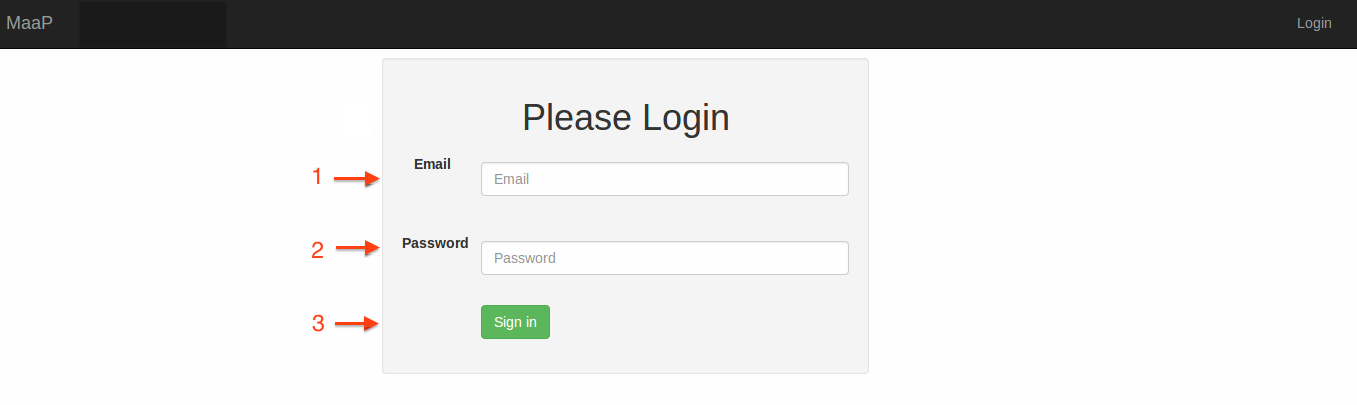
\includegraphics[width=1\textwidth]{img/login.png}
	\caption{ \label{fig:login} Pagina di login}
	\end{figure}

	\subsection{Recupero password}
	\label{recuperopassword}
	Il recupero password avviene nel caso in cui l'utente abbia perso la password. Per poter procedere con un recupero password è necessario conoscere l'\texttt{email} di registrazione. Il recupero dalla password avviene partendo dalla schermata di login (vedi figura \ref{fig:login}) cliccando sul link \texttt{Forgot your password?}, verrà proposto un \glossario{form} dove verrà richiesto di inserire l'\texttt{email} di registrazione e cliccare il pulsante di reset password. L'utente riceverà le istruzioni da seguire nella casella di posta associata all'indirizzo \texttt{email} inserito in fase di registrazione.


	\subsection{Accesso e modifica profilo personale}
	\label{modificaprofilo}
	Per accedere alla pagina di modifica del profilo, cliccare sul proprio indirizzo mail posto sulla barra dei menù e selezionare la voce \texttt{Profilo}. L'utente può modificare da qui la password di registrazione.
	% TODO inserire i passi per modificare la password di registrazione
